\documentclass[letterpaper]{memoir}
% memoir commands to define the text block geometry
\setulmarginsandblock{1in}{*}{*}
\setlrmarginsandblock{1in}{*}{*}

\usepackage{xparse}
\usepackage{blindtext}
\usepackage{enumitem}
\usepackage{graphicx}

\usepackage{amsmath,mathtools,amssymb}
% See https://texblog.net/latex-archive/maths/amsmath-matrix/ 
% for an explanation of this extention of the amsmath matrix commands.
% It's a way to enable "augmented matrices" using a new optional argument:
%
% \begin{pmatrix}[cc|c]
%     1 & 2 & 3\\
%     4 & 5 & 9
%   \end{pmatrix}
%
\makeatletter
\renewcommand*\env@matrix[1][*\c@MaxMatrixCols c]{%
  \hskip -\arraycolsep
  \let\@ifnextchar\new@ifnextchar
  \array{#1}}
\makeatother

\usepackage{bm} % bold math package

\usepackage{booktabs}
\usepackage{multirow}
\usepackage{hyperref}
\usepackage{systeme}

\usepackage{tcolorbox}
    \tcbuselibrary{skins}
    \tcbuselibrary{raster}
    \tcbuselibrary{skins}
\usepackage{tikz}
    \usetikzlibrary{arrows.meta}
\usepackage{tkz-base}
\usepackage{tkz-fct}    
\usepackage{pgfplots}
    \pgfplotsset{compat=newest}

% for inserting blanks that the students fill in
\usepackage{dashundergaps} % for \gap
\dashundergapssetup{
    teacher-mode=false, % set to true to show answers 
    gap-format=underline,
    teacher-gap-format=underline,
    gap-font={\ECFAugie\MTversion{augie}\color{black}},
    gap-numbers=false,
    gap-widen=true,
    gap-extend-percent=100, % note: making this too big might create errors
    gap-number-format=\,\textsuperscript{\normalfont(\thegapnumber)},
}

\usepackage{emerald}
\usepackage[subdued]{mathastext}% no italic for Augie anyhow
    \MTDeclareVersion[n]{lmvtt}{T1}{lmvtt}{m}{n}
    \MTfamily{augie}
    \Mathastext[augie]

    
\newcommand{\myHeadFootStyle}{\footnotesize\sffamily}
\copypagestyle{myPagestyle}{empty}
%
% FIXME
% The following header definitions do NOT work right in all cases.
% I have found that the chapter title sometimes gets picked up from
% a chapter that begins on the NEXT PAGE. Not sure what's going on.
% So I abandoned embedding the info in the header and instead updated
% \myLesson to print it out, and that seems to work find.
%
% \makeoddhead{myPagestyle}
%     {\,}
%     {\,}
%     {\myHeadFootStyle\chaptername\,\thechapter\,\,\myCurrentChapterTitle}
% \makeevenhead{myPagestyle} 
%     {\,}
%     {\,}
%     {\myHeadFootStyle\chaptername\,\thechapter\,\,\myCurrentChapterTitle}
\makeoddfoot{myPagestyle}
    {\myHeadFootStyle\myCurrentBookTitle}
    {\myHeadFootStyle\thepage}
    {\myHeadFootStyle\thechapter.\themyLessonCounter\,\,\myCurrentLessonTitle}
\makeevenfoot{myPagestyle}
    {\myHeadFootStyle\thechapter.\themyLessonCounter\,\,\myCurrentLessonTitle}
    {\myHeadFootStyle\thepage}
    {\myHeadFootStyle\myCurrentBookTitle}

\begin{document}
\pagestyle{myPagestyle}
\checkandfixthelayout

%
% I am piggy-backing off of the standard memoir document
% divisions:
%
% book    -- is for the name of my class (eg, Alg2)
% part    -- is for the semester 
% chapter -- is for units
% section -- is for the lessons in a unit
%
% To do this, I need to change the default value of various
% division-related commands. That's what the following is for.

%----- CLASS ---------
\newcommand{\myCurrentBookTitle}{}
\let\myOldBook\book
\renewcommand{\book}[1]{
    \renewcommand{\myCurrentBookTitle}{#1}
    \myOldBook{#1}
}
% I don't want roman numerals.
\makeatletter
\renewcommand*{\thebook}{\@arabic\c@book}
\makeatother
% I just want the title (not "Class 1 <title>")
\renewcommand{\printbookname}{}
\renewcommand{\booknamenum}{}
\renewcommand{\printbooknum}{}
%----- SEMESTER -------
% I don't want roman numerals.
\makeatletter
\renewcommand*{\thepart}{\@arabic\c@part}
\makeatother
%----- UNIT -----------
\renewcommand{\chaptername}{Unit}
\newcommand{\myCurrentChapterTitle}{}
\let\myOldChapter\chapter
\renewcommand{\chapter}[1]{
    \renewcommand{\myCurrentChapterTitle}{#1}
    \myOldChapter{#1}
}

%-------- LESSONS --------------
\newcounter{myLessonCounter}[chapter] 
\newcommand{\myCurrentLessonTitle}{}

\newcommand{\myLesson}[1]{
    \cleartorecto
    \stepcounter{myLessonCounter}
    \renewcommand{\myCurrentLessonTitle}{#1}
    \noindent
    \begin{minipage}[b]{0.25\textwidth}
        {
            \HUGE\bfseries\sffamily
            \thechapter.\themyLessonCounter
        }
    \end{minipage}
    \begin{minipage}[b]{0.74\textwidth}
        \begin{flushright}
            {\sffamily\chaptername\,\thechapter\,\,\myCurrentChapterTitle}\\
            \vspace{0.75\baselineskip}
            {\Huge\bfseries\sffamily#1}
        \end{flushright}
    \end{minipage}
    
    \noindent\rule{\textwidth}{1.25pt}
    \par
}

%-------- ANNOTATIONS (in boxes) --------------
% font and styling commands for
% Objectives, Voculary, Key Concepts, etc...
\newcommand{\myAnnotationStyling}{\bfseries\large}

% #1 : name of the kind of annotation (Objectives, ...)
% #2 : title text to go with the annotation
\NewDocumentEnvironment{myAnnotate}{ m m }{
    \begin{tcolorbox}[
        colbacktitle=black!15!white,
        colback=white,
        coltitle=black,
        fonttitle={\myAnnotationStyling},
        title={#1: },
        after title={\normalfont\itshape#2},
        ]
}{
    \end{tcolorbox}
}

% #1 : name of the kind of annotation 
% #2 : title 
\NewDocumentEnvironment{myTabularAnnotate}{ m m }{
    \begin{myAnnotate}{#1}{#2}
    \begin{tabular}{r|l}
}{
    \end{tabular}
    \end{myAnnotate}
}
% #1 - column 1 text
% #2 - column 2 text
\NewDocumentCommand{\myRow}{mm}{{\bfseries\itshape #1}&#2\\[1ex]}

% #1 : name of the kind of annotation 
% #2 : title 
% #3 : text before the list starts
\NewDocumentEnvironment{myListAnnotate}{ m m o }{
    \begin{myAnnotate}{#1}{#2}
    \IfValueT{#3}{#3}
    \begin{enumerate}[itemsep=0pt,]
}{
    \end{enumerate}
    \end{myAnnotate}
}
% #1 - column 1 text
% #2 - column 2 text
\NewDocumentCommand{\myItem}{mm}{\item{\bfseries\itshape #1} #2}



%----------- OBJECTIVES , VOCABULARY, CONCEPTS ---------------
\newenvironment{myObjectives}{
    \begin{myListAnnotate}{Objectives}{}
}{
    \end{myListAnnotate}
}
\newcommand{\myObjective}[2]{
    \myItem{#1}{#2}
}

\newenvironment{myVocabulary}{
    \begin{myTabularAnnotate}{Vocabulary}{}
}{
    \end{myTabularAnnotate}
}
\newcommand{\myDefinition}[2]{
    \myRow{#1}{#2}
}

\NewDocumentEnvironment{myConcept}{m}{
    \begin{myAnnotate}{Key Concept}{#1}
}{
    \end{myAnnotate}
}

\NewDocumentEnvironment{myConceptSteps}{m}{
    \begin{myListAnnotate}{Key Concept}{#1}[Follow these steps.]
}{
    \end{myListAnnotate}
}
\newcommand{\myStep}[2]{
    \myItem{#1.}{#2}
}

%----------- EXAMPLEs ---------------
\newcounter{myExampleCounter}[myLessonCounter] 

% #1 A statement of the example problem.
%
\NewDocumentEnvironment{myExample}{m}{%
    \begin{tcolorbox}[
        enhanced,
        sharp corners, 
        colback=white,
        boxrule=0pt,
        borderline={0.5pt}{0pt}{black,dashed},
        ]
        \stepcounter{myExampleCounter}
        {\myAnnotationStyling Example \themyExampleCounter:} #1
        \tcblower
}{
    \end{tcolorbox}
}







\book{Pre-AP Algebra 2}
\part{Fall Semester}
\chapter{Introduction to Relations and Functions}
\myLesson{This is a lesson}

\begin{myObjectives}
    \myObjective{listen}{to the teacher}
    \myObjective{take}{notes in my notebook}
    \myObjective{see}{farther than anyone else}
\end{myObjectives}

\begin{myVocabulary}
    \myDefinition{vertical}{up and down}
    \myDefinition{horizontal}{left and right}
    \myDefinition{foo}{an arbitrary name}
\end{myVocabulary}

\begin{myConcept}{To do this\dots}
    then what you need to do is that.
\end{myConcept}

\begin{myConceptSteps}{To do this\dots}
    \myStep{foo}{First you foo.}
    \myStep{bar}{Then you bar.}
    \myStep{baz}{Finally you baz.}
\end{myConceptSteps}

\begin{myExample}{Do something!}
    foo
\end{myExample}

\begin{myExample}{Do something!}
    \vspace{.05in}
\end{myExample}

\myLesson{This is another lesson}

foo bar baz


\chapter{Another unit ggg}
\myLesson{This is another lesson g}

\blindtext

\begin{myExample}{Do something!}
    foo
\end{myExample}

\begin{myExample}{Do something!}
    \vspace{.05in}
\end{myExample}

\begin{myExample}{Do something!}
    \begin{center}
        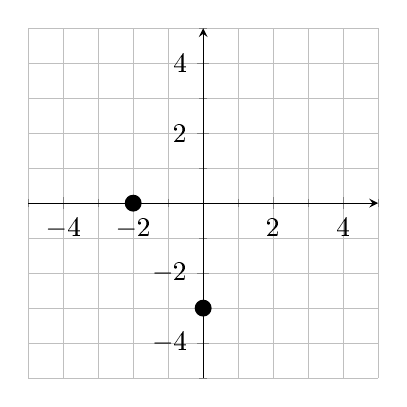
\begin{tikzpicture}
            \begin{axis}[
                width=2.75in,
                grid=both,
                axis x line = middle,axis y line = middle,
                axis equal image,
                xtick distance = 2, ytick distance = 2,
                xmin = -5, xmax = 5,
                ymin = -5, ymax = 5,
                minor tick num = 1,
                ]
                \addplot[
                    only marks,
                    mark=*,
                    mark size = 0.1cm,
                    ] coordinates { (0,-3) (-2,0) };
            \end{axis}
        \end{tikzpicture}
    \end{center}
\end{myExample}

\chapter{final unit yyy}
\blindtext

\end{document}